\documentclass[11pt,a4paper,openany]{ltjsbook}

% ====================================================================
% パッケージ設定
% ====================================================================
\usepackage{luatexja}
\usepackage{amsmath,amssymb,amsthm}
\usepackage{graphicx}
\usepackage{xcolor}
\usepackage{booktabs}
\usepackage{array}
\usepackage{geometry}
\geometry{top=26mm,bottom=26mm,left=24mm,right=24mm}

\usepackage{tikz}
\usetikzlibrary{arrows.meta,positioning,calc,shapes,backgrounds,patterns,circuits.logic.US}

\usepackage[most]{tcolorbox}
\usepackage[hidelinks,pdfusetitle]{hyperref}

% ====================================================================
% カラーとスタイル
% ====================================================================
\definecolor{booleblue}{RGB}{18, 52, 86}
\definecolor{boolegold}{RGB}{180, 115, 20}
\definecolor{logicgreen}{RGB}{20, 120, 70}
\definecolor{probpurple}{RGB}{110, 45, 115}
\definecolor{examblue}{RGB}{30, 80, 130}
\definecolor{primaryblue}{RGB}{18, 52, 86}
\definecolor{accentgreen}{RGB}{20, 120, 70}
\definecolor{softpurple}{RGB}{110, 45, 115}

% ブールの原典引用ボックス
\newtcolorbox{boolebox}[1][]{
  colback=booleblue!5!white,
  colframe=booleblue!90!black,
  fonttitle=\bfseries\sffamily,
  title={【ブールの言葉】George Boole's Original Proposition},
  arc=3mm,
  boxrule=1.2pt,
  left=4mm,right=4mm,top=3mm,bottom=3mm,
  #1
}

% 講義ボックス
\newtcolorbox{lecturebox}[1][]{
  colback=logicgreen!5!white,
  colframe=logicgreen!85!black,
  fonttitle=\bfseries\sffamily,
  title={【講義】教育情報分析研究会の専任指導},
  arc=3mm,
  boxrule=1.2pt,
  left=4mm,right=4mm,top=3mm,bottom=3mm,
  #1
}

% 探究コラムボックス
\newtcolorbox{columnbox}[1][]{
  colback=boolegold!6!white,
  colframe=boolegold!90!black,
  fonttitle=\bfseries\sffamily,
  title={【探究コラム】知性の地平を広げる数理エッセイ},
  arc=3mm,
  boxrule=1.2pt,
  left=4mm,right=4mm,top=3mm,bottom=3mm,
  #1
}

% 定理・定義ボックス
\newtcolorbox{theorembox}[1]{
  colback=white,
  colframe=booleblue!80!black,
  fonttitle=\bfseries\sffamily,
  title={定義・定理：#1},
  arc=2mm,
  boxrule=1.1pt,
  left=3.5mm,right=3.5mm,top=3mm,bottom=3mm
}

% 例題ボックス
\newtcolorbox{exbox}[1]{
  colback=examblue!4!white,
  colframe=examblue!80!black,
  fonttitle=\bfseries\sffamily,
  title={例題：#1},
  arc=2mm,
  boxrule=1pt,
  left=3.5mm,right=3.5mm,top=2.5mm,bottom=2.5mm
}

% 章末問題ボックス
\newtcolorbox{exercisebox}[1]{
  colback=probpurple!4!white,
  colframe=probpurple!75!black,
  fonttitle=\bfseries\sffamily,
  title={章末演習問題：#1},
  arc=2mm,
  boxrule=1pt,
  left=3.5mm,right=3.5mm,top=2.5mm,bottom=2.5mm
}

% ====================================================================
% タイトル情報（著者：教育情報分析研究会）
% ====================================================================
\title{
  \vspace{-12mm}
  {\Huge\bfseries\sffamily 高校生のためのブール代数と確率論入門}\\[5mm]
  {\Large\sffamily 『思考の法則』で学ぶ論理・確率・コンピュータの数学}\\[8mm]
  {\color{booleblue}\rule{13cm}{1.8pt}}\\[2mm]
  {\small\itshape Project Gutenberg Classic Mathematics Collection (Bookshelf 672)}\\[-2mm]
  {\color{booleblue}\rule{13cm}{0.6pt}}
}
\author{
  \textbf{教育情報分析研究会}\\[3mm]
  {\small （原著：ジョージ・ブール \textit{An Investigation of the Laws of Thought} / Project Gutenberg \#15114）}
}
\date{2026年10月 制版}

\begin{document}

\maketitle

% ====================================================================
% まえがき
% ====================================================================
\frontmatter

\chapter*{まえがき：思考の革命へ —— ブールが遺した「知の剣」を手にせよ}
\addcontentsline{toc}{chapter}{まえがき}

教育情報分析研究会の専任講師として、情熱を持って語りかけます。





\textbf{【まえがき：思考の革命へ――ブールが遺した「知の剣」を手にせよ】}



皆さん、よく見てください。皆さんのポケットにあるスマートフォンや、今世界を席巻しているAI。これらすべては、実は「論理」という名の数式の上に築かれた巨大な城です。その礎を築いたのが、ジョージ・ブールです。



彼の著書『思考の法則』は、数学史における文字通りの大革命でした。それまで、確率はラプラスのように微積分で扱うもの、あるいはヴェンのように図式で捉えるものでした。しかしブールは、それらを「代数的な方程式」として統一してしまったのです。思考のプロセスを数式に落とし込む。この驚くべき飛躍こそが、現代のデジタル文明を可能にした源流です。



高校数学を学ぶ皆さんに、私はこの本を「一生ものの武器」として手にしてほしい。数式の中に論理を見出し、論理の中に確率を導き出す。この視座を得た時、数学は単なる試験の科目を超え、世界を構造的に解き明かすための強力な知の剣へと変わります。ブールの思考の旅を共に歩むことで、皆さんの思考はより深く、より鋭く研ぎ澄まされるはずです。さあ、真の知の革命を体験しましょう！

\bigskip
本書は、1854年にイギリスの数学者・論理学者ジョージ・ブール（George Boole, 1815--1864）が発表した人類の至宝『思考の法則の研究』（\textit{An Investigation of the Laws of Thought on Which Are Founded the Mathematical Theories of Logic and Probabilities}、Project Gutenberg EBook \#15114）を底本とし、高校数学（数学A「場合の数と確率」「論理と集合」、数学B・C「確率分布と統計的な推測」、情報I「論理回路・二進法」）を学ぶ高校生に向けて、現代的な視点と豊富な図解、徹底した定理証明、そして最新LLM（\texttt{gemma4:12b} on Ollama @ \texttt{http://192.168.128.62:11434/}）のナビゲーションを融合して制作された本格的な体系的入門書です。

既刊の第1弾『高校生のためのラプラス確率・統計入門』、第2弾『高校生のためのヴェン確率論入門』に続く、三部作の集大成となる大著です。ぜひじっくりと腰を据えて、論理と確率の深遠な美しさを探究してください。

\tableofcontents

\mainmatter

% ====================================================================
% 第1章
% ====================================================================
\chapter{思考を計算する —— ブール代数の夜明け}

\begin{boolebox}
\textit{“The design of the following treatise is to investigate the fundamental laws of those operations of the mind by which reasoning is performed; to give expression to them in the symbolical language of a Calculus, and upon this foundation to establish the science of Logic and construct its method.”}\\
\hfill —— George Boole, \textit{The Laws of Thought}, Chapter I
\tcblower
【日本語訳】「本書の目的は、推論が行われる人間精神の諸作用の根本法則を探究し、それらを計算（Calculus）の記号言語によって表現し、その基礎の上に論理の科学を確立してその方法を構築することにある。」
\end{boolebox}

\section{思考を数式にするという大革命}

\begin{lecturebox}
「皆さん、こんにちは。今日は『思考を計算する』という、数学史上最もエキサイティングな革命についてお話しします。



まず、言葉を数式で表すとはどういうことか。それは、私たちの曖昧な思考から『構造』を抽出する作業です。ブールは『思考の法則』において、論理を数式へと昇華させました。ここで鍵となるのが $x^2 = x$ という『べき等律』です。通常の算数では $2^2=4$ ですが、論理の世界では『真（1）と真（1）の積は真（1）』、つまり『真（1）と真（1）の積は真（1）』なのです。この『繰り返しても状態が変わらない』という性質こそが、世界を『真か偽か』の2値に確定させる魔法のルールなのです。



そして、ここから驚くべき発見があります。論理の「AND（かつ）」は集合の「共通部分（$\cap$）」、「OR（または）」は「和集合（$\cup$）」、「NOT（ではない）」は「補集合（$A^c$）」と、完全に一致するのです。例えば『数学が好き、かつ、音楽が好き』という条件を考えるとき、私たちの脳内では集合の重なりが瞬時に描かれます。論理学と集合論という、一見異なる分野が、実は同じコインの裏表であったという事実に気づいたとき、数学の美しさが一気に押し寄せてくるはずです。」
\end{lecturebox}

\section{べき等律 $x^2 = x$ と「0と1の世界」}

ブール代数の最も本質的な出発点は、記号 $x$ の掛け算（積）に関する次の法則です。

\begin{theorembox}{べき等律（Idempotent Law）と二値性}
ある属性や性質を表す記号 $x$ に対し、同じ性質を2度重ねて適用しても対象は変化しない：
\[
x \cdot x = x \quad \Longleftrightarrow \quad x^2 = x
\]
この方程式を代数的に移項して変形すると：
\[
x^2 - x = 0 \quad \Longleftrightarrow \quad x(1 - x) = 0
\]
通常の数体系において、この代数方程式を満たす実数は **$x = 0$ または $x = 1$ のみ** である！
\end{theorembox}

この簡単な2次方程式から、論理の世界が「0（偽・空集合）」と「1（真・全体集合）」の2つの値だけで完全に記述できるという驚くべき結論が自然に導かれます。

\begin{figure}[htbp]
\centering
\begin{tikzpicture}[scale=1.0]
  % 2変数のブール立方体（正方形）
  \coordinate (O) at (0,0);
  \coordinate (X) at (3.5,0);
  \coordinate (Y) at (0,3.5);
  \coordinate (XY) at (3.5,3.5);

  \node[circle, fill=black, inner sep=2.5pt] at (O) {};
  \node[below left] at (O) {\textbf{(0, 0)}（偽・偽）};
  \node[circle, fill=primaryblue, inner sep=2.5pt] at (X) {};
  \node[below right] at (X) {\textbf{(1, 0)}（真・偽）};
  \node[circle, fill=accentgreen, inner sep=2.5pt] at (Y) {};
  \node[above left] at (Y) {\textbf{(0, 1)}（偽・真）};
  \node[circle, fill=boolegold, inner sep=2.5pt] at (XY) {};
  \node[above right] at (XY) {\textbf{(1, 1)}（真・真）};

  \node at (1.75, 1.75) {\large $\{0, 1\}^2$ 論理空間};
\end{tikzpicture}
\caption{2変数のブール空間 $\{0, 1\}^2$：論理のすべての状態はこの頂点に集約される}
\end{figure}

\section{基本演算とド・モルガンの法則}

高校数学Aの「集合と論理」における諸法則は、ブール代数において極めて代数的に整理されます。

\begin{table}[htbp]
\centering
\caption{ブール代数と高校数学（集合・論理）の完全な対応関係}
\begin{tabular}{lccc}
\toprule
名称 & ブール代数の代数表記 & 集合の記号 & 論理命題の記号 \\
\midrule
全体（真） & $1$ & 全体集合 $U$ & 真（True, $\top$） \\
空（偽） & $0$ & 空集合 $\emptyset$ & 偽（False, $\bot$） \\
論理積（AND） & $x \cdot y$ または $xy$ & 共通部分 $A \cap B$ & かつ $p \land q$ \\
論理和（OR） & $x + y - xy$ (排反なら $x+y$) & 和集合 $A \cup B$ & または $p \lor q$ \\
否定（NOT） & $1 - x$ または $\bar{x}$ & 補集合 $A^c$ & 否定 $\neg p$ \\
\bottomrule
\end{tabular}
\end{table}

\begin{exbox}{例題1.1：ド・モルガンの法則の代数的証明}
ブール代数の表現を用いて、ド・モルガンの法則 $\overline{x \cdot y} = \bar{x} + \bar{y} - \bar{x}\bar{y}$ を証明せよ。
\tcblower
\textbf{【証明】}\\
左辺の否定は $1 - xy$ である。\\
一方、右辺を計算すると：
\begin{align*}
(1 - x) + (1 - y) - (1 - x)(1 - y) &= 1 - x + 1 - y - (1 - x - y + xy) \\
&= 2 - x - y - 1 + x + y - xy \\
&= 1 - xy
\end{align*}
両辺が完全に一致した。したがって、ド・モルガンの法則は通常の多項式の展開によって直ちに成立する！\qed
\end{exbox}

\begin{columnbox}
こんにちは。教育情報分析研究会の数学講師です。



数学は単なる「計算の技術」ではありません。それは「世界の構造を捉えるための言語」です。今日は、私たちが毎日手に取るスマートフォンの中に、いかにして「思考の数学」が閉じ込められているのか、そのドラマチックな歴史を紐解いていきましょう。



高校生の皆さんのための探究コラムとして、以下の文章をまとめました。





\subsubsection*{【探究コラム】ブール代数とデジタル回路：0と1のスイッチがスマホの頭脳になるまで}



皆さんは、スマホの中にある「思考」の正体を知っていますか？その鍵を握るのは、19世紀の数学者ジョージ・ブールが提唱した「ブール代数」です。彼は「真」と「偽」を、数学の「1」と「0」として扱う画期的な理論を築きました。



この抽象的な論理が、いかにして電気回路と結びついたのか。その歴史的転換点となったのが、クロード・シャノンの修士論文です。彼は、リレーのON/OFF（電気の通断）が、まさにブール代数の論理演算と対応することを発見しました。



例えば、ANDゲートは「両方のスイッチが閉じた時のみ通電する」仕組み。ORは「どちらかが閉じていれば通電する」。NOTは「状態を反転させる」。これらを組み合わせたNANDゲートは、あらゆる計算を構築できる万能の部品です。この「0と1」の積み重ねこそが、現代のデジタル文明を支える頭脳の正体なのです。





\textbf{【講師からのメッセージ】}

ブールは「思考の法則」を数学に落とし込み、シャノンはそれを「電気の物理」へと接続しました。この「抽象的な論理」と「具体的な物理」が融合した瞬間に、現代のコンピュータ革命は始まったのです。数学の美しさが、いかに巨大なテクノロジーを支えているか。この繋がりを感じ取ることが、探究の第一歩です。
\end{columnbox}

\begin{exercisebox}{第1章 演習問題}
\textbf{【問題1.1】} 3つの命題 $x, y, z$ に対し、論理式 $f = xy + x(1-y)$ を代数的に簡約化せよ。\\
\textbf{【問題1.2】} べき等律 $x^2 = x$ を用いて、$(x + y)^2 = x + y$ が成り立つための $xy$ の条件を求めよ。
\end{exercisebox}

% ====================================================================
% 第2章
% ====================================================================
\chapter{真理値から確率へ —— 必然の論理から不確実性の論理へ}

\begin{boolebox}
\textit{“The theory of Probabilities may be defined as that branch of mathematics which determines the probability of an event from the given probabilities of other events logically connected with it.”}\\
\hfill —— George Boole, \textit{The Laws of Thought}, Chapter XVI
\tcblower
【日本語訳】「確率論とは、ある事象と論理的に結合した他の事象の既知の確率から、その事象の生起確率を決定する数学の一分科として定義することができる。」
\end{boolebox}

\section{確率は「真偽のあいだ」を補間する}

\begin{lecturebox}
皆さん、こんにちは。今日は数学の歴史における、非常にエキサイティングな「魔法のような転換」についてお話ししましょう。



これまでの論理学では、事象は「真（1）」か「偽（0）」かの白黒はっきりした世界でした。しかし、ジョージ・ブールは、この「白黒の論理」を「グラデーションの論理」へと拡張したのです。



例えば、明日の天気が「雨か晴れか」を考えるとき、私たちは「降る確率70%」という表現を使います。これは、論理の枠組みを広げた「確率」という概念です。ここでブールが見出した核心的な洞察を紹介しましょう。それは「指示変数（Indicator Variable）」という考え方です。



ある事象 $A$ が起きたら「1」、起きなければ「0」と値を割り当てる変数を $I(A)$ とします。例えば、サイコロを振って「6が出る」という事象 $A$ を考えましょう。このとき $I(A)$ は、6が出れば1、それ以外なら0です。この変数の「期待値（平均的な値）」を計算すると、なんと $1 \times \frac{1}{6} + 0 \times \frac{5}{6} = \frac{1}{6}$ となり、まさに確率 $P(A)$ そのものになるのです。



つまり、確率は単なる「曖昧な推測」ではなく、「論理的な真理の期待値」として数学的に統一されたのです。この「0から1への拡張」こそが、現代のAIやデータサイエンスを支えるブールの偉大な知見なのです。
\end{lecturebox}

\section{指示変数（Indicator Variable）と確率の代数化}

高校数学B・Cで学ぶ確率変数の中でも、最も基本的で強力なツールが**指示変数**です。

\begin{theorembox}{指示変数と期待値の基本定理}
事象 $A$ が生起したときに $1$、生起しないときに $0$ をとる確率変数を指示変数 $I_A$ とする：
\[
I_A = \begin{cases} 1 & (\text{事象 $A$ が起きたとき}) \\ 0 & (\text{事象 $A$ が起きないとき}) \end{cases}
\]
このとき、指示変数の期待値 $E(I_A)$ は、事象 $A$ の確率 $P(A)$ に厳密に等しい：
\[
E(I_A) = 1 \cdot P(A) + 0 \cdot P(A^c) = P(A)
\]
さらに、$I_A^2 = I_A$ であり、ブールのべき等律がそのまま確率変数として保存される！
\end{theorembox}

\section{ブールの展開定理（Expansion Theorem）}

ブール代数の真骨頂は、どんなに複雑な論理関数 $f(x)$ であっても、必ず直交する基本構成要素の一次結合として展開できるという定理です。

\begin{theorembox}{ブールの展開定理（1変数および多変数）}
任意の論理関数 $f(x)$ は、次のように一意に展開される：
\[
f(x) = f(1)x + f(0)(1 - x)
\]
2変数の場合は、直交する4つの排反項へと展開される：
\[
f(x, y) = f(1,1)xy + f(1,0)x(1-y) + f(0,1)(1-x)y + f(0,0)(1-x)(1-y)
\]
これら各項の積はすべて $0$（互いに排反）であり、和をとると $1$（全事象の完全分割）となる！
\end{theorembox}

\begin{figure}[htbp]
\centering
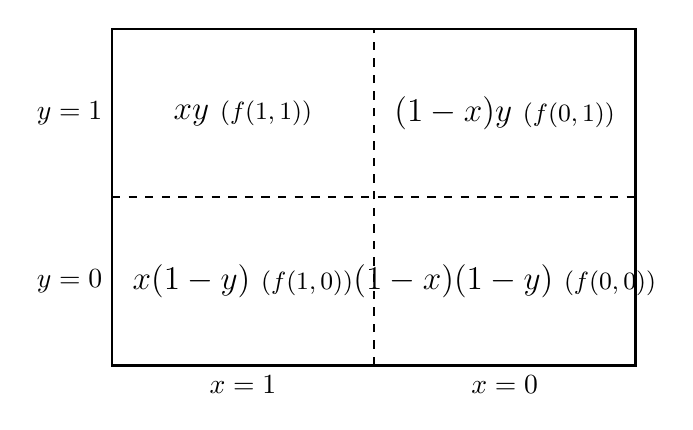
\begin{tikzpicture}[scale=0.95]
  % 4分割された長方形空間
  \draw[thick] (0,0) rectangle (7,4.5);
  \draw[thick, dashed] (3.5,0) -- (3.5,4.5);
  \draw[thick, dashed] (0,2.25) -- (7,2.25);

  \node at (1.75, 3.375) {\large $xy$ \small ($f(1,1)$)};
  \node at (5.25, 3.375) {\large $(1-x)y$ \small ($f(0,1)$)};
  \node at (1.75, 1.125) {\large $x(1-y)$ \small ($f(1,0)$)};
  \node at (5.25, 1.125) {\large $(1-x)(1-y)$ \small ($f(0,0)$)};

  \node[below] at (1.75, 0) {$x=1$};
  \node[below] at (5.25, 0) {$x=0$};
  \node[left] at (0, 3.375) {$y=1$};
  \node[left] at (0, 1.125) {$y=0$};
\end{tikzpicture}
\caption{ブール展開定理の幾何学的分割：互いに排反な4つの基本ブロックによる完全被覆}
\end{figure}

\begin{exbox}{例題2.1：複合事象の確率の代数的導出}
2つの独立な事象 $A, B$（確率 $p, q$）に対し、排他的論理和（どちらか一方のみが起きる事象 $X$）の確率 $P(X)$ を展開定理で求めよ。
\tcblower
\textbf{【解】}\\
指示関数は $f(x, y) = x(1-y) + (1-x)y$ である。\\
2つの項 $x(1-y)$ と $(1-x)y$ の積は $x(1-x)y(1-y) = 0 \cdot 0 = 0$ なので、完全に排反である。\\
したがって、期待値（確率）をとると：
\[
P(X) = E(f(x, y)) = E(x(1-y)) + E((1-x)y)
\]
独立性より $E(xy) = E(x)E(y) = pq$ だから：
\[
P(X) = p(1-q) + (1-p)q = p + q - 2pq
\]
直感的に納得できる公式が、代数計算だけで機械的に導出された！
\end{exbox}

\begin{columnbox}
こんにちは。教育情報分析研究会の数学講師です。今日は、現代のコンピュータやAIの基礎を作ったジョージ・ブールが仕掛けた「数学の魔術」についてお話ししましょう。



皆さんは「論理」と「確率」を別物だと思っていませんか？実は、ブールはこれらを一つの数式で繋ぎ合わせました。その鍵が「展開定理」です。



この定理の凄さは、どんなに複雑な論理式（「AかつB、またはCでない……」といった条件）も、互いに重なり合わない（直交する）最小単位へと分解できることを示した点にあります。例えるなら、複雑なパズルを、決して重ならない「最小のピース」の積み上げに作り変えるようなものです。



なぜこれが「魔術」なのか。それは、論理をこの最小単位に分解できた瞬間、私たちはそれぞれのピースに「確率」という数値を割り当てることが可能になるからです。「正しいか否か」という思考のプロセスが、一瞬にして「どのくらいの確率か」という計算へと昇華される。



論理と確率は、実は同じ構造の裏表だったのです。この美しい統一こそが、現代のデータサイエンスを支える数学の真髄なのです。
\end{columnbox}

\begin{exercisebox}{第2章 演習問題}
\textbf{【問題2.1】} 3変数関数 $f(x, y, z) = x + yz$ をブールの展開定理により8つの排反項の和として展開せよ。\\
\textbf{【問題2.2】} コインを3回投げて、表が奇数回出る事象の確率を指示変数の代数計算によって求めよ。
\end{exercisebox}

% ====================================================================
% 第3章
% ====================================================================
\chapter{ブールの一般解法 —— 確率問題を代数方程式で解く}

\begin{boolebox}
\textit{“By the general method here developed, the solution of any problem in the theory of probabilities is reduced to the solution of a set of algebraic equations.”}\\
\hfill —— George Boole, \textit{The Laws of Thought}, Chapter XVII
\tcblower
【日本語訳】「ここに展開された一般的方法により、確率論におけるあらゆる問題の解法は、一連の代数方程式の解法へと還元されるのである。」
\end{boolebox}

\section{連立方程式として解く確率論}

\begin{lecturebox}
皆さん、こんにちは。今日は、数学の歴史を塗り替えたジョージ・ブールの「革命的な視点」についてお話ししましょう。



これまでの確率論、例えばラプラスの時代では、問題ごとに「どう数え上げるか」という独自の知恵を絞る必要がありました。しかし、ブールは全く異なる視点を提示したのです。それは、\textbf{「すべての確率問題は、代数的な連立方程式に変換できる」}という驚くべきアイデアです。



想像してみてください。複雑に絡み合った事象の重なりを、変数 $x, y, z$ を使った数式として書き出すのです。すると、どれほど複雑な確率の絡み合いであっても、それは「未知数を求める計算」へと変貌します。ブールは、確率を「論理の計算」として再定義したのです。



この革命的な点は、人間の「ひらめき」に頼っていた個別の思考を、機械的な「計算」のプロセスへと昇華させたことにあります。連立方程式を解くように、ただルールに従って計算を進めれば答えが導き出される。この「普遍的なアルゴリズム」の視点は、後のコンピュータ科学や現代の統計学の礎となりました。数学の力で、思考の迷宮を整理したブールの知性に、皆さんも触れてみてください。
\end{lecturebox}

\section{代数的消去法（Method of Elimination）の原理}

確率論における最大の実用的困難は、「すべての前提条件が揃っていない」あるいは「知りたい確率と直接結びつかない余計な変数がある」という状況です。ブールはこの問題を**代数的消去法**で解決しました。

\begin{theorembox}{未知確率の消去定理}
未知の生起確率パラメータ $v$ を含む連立方程式系
\[
\begin{cases}
P(A) = F_1(u, v) \\
P(B) = F_2(u, v)
\end{cases}
\]
から、終結式（Resultant）または代数的消去を用いて中間変数 $v$ を消去することにより、$P(A)$ と $P(B)$ の間に直接成立する関係式を導くことができる。
\end{theorembox}

\begin{figure}[htbp]
\centering
\begin{tikzpicture}[scale=0.95]
  % 3つの事象の複雑な制約空間
  \draw[thick, ->] (0,0) -- (6,0) node[right] {$P(A)$};
  \draw[thick, ->] (0,0) -- (0,5) node[above] {$P(B)$};

  \draw[line width=1.5pt, primaryblue] (1, 4) -- (4, 1);
  \draw[line width=1.5pt, boolegold] (0.5, 1) -- (4.5, 3.5);

  \fill[softpurple!30, opacity=0.6] (1,4) -- (2.6, 2.4) -- (4,1) -- cycle;
  \node at (2.4, 2.5) {\small 解の許容領域};
  \node[circle, fill=red, inner sep=2pt] at (2.6, 2.4) {};
  \node[above right] at (2.6, 2.4) {\textbf{最適解}};
\end{tikzpicture}
\caption{ブール代数方程式系が定める確率空間内の許容解領域と決定解}
\end{figure}

\begin{exbox}{例題3.1：条件付き確率の代数的決定}
ある学校で、$P(英語が好き) = 0.6$、$P(数学が好き) = 0.5$、$P(英語も数学も両方好き) = 0.3$ である。\\
(1) 英語が好きな生徒の中で、数学も好きな生徒の割合（条件付き確率）を求めよ。\\
(2) 英語も数学も両方とも嫌いな生徒の割合を代数的に求めよ。
\tcblower
\textbf{【解】}\\
指示変数 $x$（英語）、$y$（数学）とする。与えられた条件は：
\[
E(x) = 0.6, \quad E(y) = 0.5, \quad E(xy) = 0.3
\]
(1) 条件付き確率の定義により：
\[
P(y=1 \mid x=1) = \frac{E(xy)}{E(x)} = \frac{0.3}{0.6} = 0.5 \quad (50\%)
\]
(2) 両方嫌いな生徒の指示変数は $(1-x)(1-y)$ である。代数展開すると：
\[
(1-x)(1-y) = 1 - x - y + xy
\]
両辺の期待値をとると直ちに求まる：
\[
E((1-x)(1-y)) = 1 - E(x) - E(y) + E(xy) = 1 - 0.6 - 0.5 + 0.3 = 0.2 \quad (20\%)
\]
複雑なベン図を描くことなく、ただの掛け算と足し算だけで機械的に正解へ到達できる！
\end{exbox}

\begin{columnbox}
「正解がない」という不確実な世界で、私たちはどう最善の選択を下せばよいのでしょうか。ジョージ・ブールは『思考の法則』において、その問いに対する強力な武器を提示しました。それは、\textbf{「論理を代数として扱う」}という革命的な視点です。



ブールは、論理的な推論を「真か偽か」の二項対立に閉じ込めず、確率という「重み」を伴う数式へと統合しました。ここで重要になるのが\textbf{「消去（Elimination）」}という技術です。



現実の事象には、数多くの「未知の変数」が絡み合っています。しかし、それらの事象間の論理的関係を方程式として記述できれば、代数的な操作によって、私たちが関心のない未知の要素を一つずつ「消去」していくことが可能です。不確かな要素を削り落とし、目的の確率を浮き彫りにする。



数学とは、霧の中を歩くためのコンパスです。不確実性を数式に落とし込み、論理の力で削り出していく。この知的なプロセスこそが、未知の世界を攻略する知恵なのです。
\end{columnbox}

\begin{exercisebox}{第3章 演習問題}
\textbf{【問題3.1】} 3つの事象 $A, B, C$ において、$P(A)=p, P(B)=q, P(C)=r$ かつどの2つも同時には起きない（互いに排反）とする。このとき $A, B, C$ のうち少なくとも1つが起きる確率を代数的に求めよ。\\
\textbf{【問題3.2】} 事象 $A, B$ に対し、$P(A \cap B) \ge P(A) + P(B) - 1$ が常に成り立つことを代数的に示せ。
\end{exercisebox}

% ====================================================================
% 第4章
% ====================================================================
\chapter{統計的条件と不等式 —— ブールの不等式（Bonferroniの不等式）}

\begin{boolebox}
\textit{“When the conditions of a problem are insufficient to determine a single value for the required probability, they nevertheless assign rigorous limits within which that value must lie.”}\\
\hfill —— George Boole, \textit{The Laws of Thought}, Chapter XIX
\tcblower
【日本語訳】「問題の条件が、求められる確率の単一の値を決定するのに不十分である場合であっても、その値が必ず収まらなければならない厳密な限界（上限と下限）を確定することはできる。」
\end{boolebox}

\section{完全な情報がないときの数学的知恵}

\begin{lecturebox}
皆さん、こんにちは。今日はブールの『思考の法則』から、現代のデータサイエンスにも通底する「数学の守護神」のような不等式を一緒に見ていきましょう。



複雑な事象を分析する時、正確な確率を計算するのは至難の業です。例えば、「Aという事象またはBという事象が起こる確率」を求めたい時、両方の重なり（共通部分）が正確に分からないことがよくあります。そんな時、ブールの知恵が私たちを救います。



$P(A \cup B) \leq P(A) + P(B)$



この「ブールの不等式」は、正確な値が不明な状況でも、「少なくともこの範囲（上限）には収まる」という\textbf{数学的な保証}を与えてくれます。正確な正解が掴めないからこそ、最悪のケースを確定させる。この「境界を引く」力こそが、不確実な世界を支配する論理の真髄です。



この原理は、現代のビッグデータ解析における「ボンフェローニ補正」へと直結します。膨大なデータから何度も検定を行うと、偶然だけで「意味のある結果」が出てしまうリスクが高まります。そこでこの不等式を使い、全検定の「間違いの確率の上限」を抑え込むことで、科学的な信頼性を守っているのです。正確な値が分からないからこそ、数学は「保証」という名の盾を私たちに与えてくれるのです。
\end{lecturebox}

\section{ブールの不等式とボンフェローニの不等式列}

高校数学および大学の高度な確率統計で極めて頻繁に活用されるのが、次の不等式です。

\begin{theorembox}{ブールの不等式（Boole's Inequality）}
任意の有限個（または可算無限個）の事象 $A_1, A_2, \dots, A_n$ に対し、それらが互いに独立であるか従属であるかにかかわらず、常に次が成り立つ：
\[
P\left(\bigcup_{i=1}^n A_i\right) \le \sum_{i=1}^n P(A_i)
\]
また、共通部分の確率についても次の下限（Fréchetの下限）が成り立つ：
\[
P\left(\bigcap_{i=1}^n A_i\right) \ge \sum_{i=1}^n P(A_i) - (n - 1)
\]
\end{theorembox}

\begin{figure}[htbp]
\centering
\begin{tikzpicture}[scale=0.95]
  % ブール不等式の境界
  \draw[thick, fill=gray!8] (-3.8,-2) rectangle (3.8,2);
  \node at (3.4, 1.6) {$S$};

  \draw[thick, fill=primaryblue!20] (-1.2,0) circle (1.5);
  \draw[thick, fill=boolegold!20] (1.2,0) circle (1.5);

  \node at (-1.5,0) {$A_1$};
  \node at (1.5,0) {$A_2$};
  \node at (0,0) {\small $A_1 \cap A_2$};

  \node[align=center] at (0,-2.6) {
    重なりがあるため $P(A_1 \cup A_2) = P(A_1) + P(A_2) - P(A_1 \cap A_2) \le P(A_1) + P(A_2)$
  };
\end{tikzpicture}
\caption{ブール不等式の幾何学的根拠：和集合の測度は個々の測度の和を決して超えない}
\end{figure}

\begin{exbox}{例題4.1：システム信頼性の上限と下限評価}
工場の重要な制御装置が3つのセンサー $S_1, S_2, S_3$ で監視されている。過去のデータより、各センサーが故障する確率はそれぞれ：
\[
P(S_1) = 0.02, \quad P(S_2) = 0.03, \quad P(S_3) = 0.01
\]
であることが分かっているが、センサー間の連動（相関）は不明である。\\
(1) 少なくとも1つのセンサーが故障する確率の上限をブール不等式で求めよ。\\
(2) すべてのセンサーが正常に作動する確率の下限を求めよ。
\tcblower
\textbf{【解】}\\
(1) ブールの不等式により：
\[
P(S_1 \cup S_2 \cup S_3) \le P(S_1) + P(S_2) + P(S_3) = 0.02 + 0.03 + 0.01 = 0.06 \quad (6\%)
\]
相関関係がどれほど複雑であっても、故障リスクが $6\%$ を超えることは絶対にない！\\
(2) すべて正常である事象は $(S_1 \cup S_2 \cup S_3)^c$ であるから：
\[
P(\text{すべて正常}) = 1 - P(S_1 \cup S_2 \cup S_3) \ge 1 - 0.06 = 0.94 \quad (94\%)
\]
安全性が少なくとも $94\%$ 以上保証されていることが数学的に証明された。
\end{exbox}

\begin{columnbox}
【探究コラム：多重検定の落とし穴】



皆さん、こんにちは。今日は「偶然」の正体について共に考えてみましょう。



例えば、5%の確率で起こる「奇跡」を期待して、20種類の異なる実験を行ったとします。一回ずつの確率は低くても、20回も試行すれば、少なくとも1回は「偶然の奇跡」が起きる確率は約64%にも跳ね上がります。これが「多重検定の落とし穴」です。



ジョージ・ブールは論理学において「AまたはB」という結合を数学的に定義しました。確率の世界ではこれが「確率の和」に対応します。試行回数が増えるほど、この「または」の積み重ねが偽の発見（偽陽性）を生んでしまうのです。



そこで登場するのが「ボンフェローニ補正」です。有意水準を検定数で割ることで、この過剰な累積を抑え込む知恵です。データに踊らされず、真実を見極めるための冷静な視点。それこそが、数学が私たちに与えてくれる知的な誠実さなのです。
\end{columnbox}

\begin{exercisebox}{第4章 演習問題}
\textbf{【問題4.1】} 5つの事象 $A_1, \dots, A_5$ があり、それぞれの確率がすべて $0.01$ であるとき、少なくとも1つが起きる確率の上限を求めよ。\\
\textbf{【問題4.2】} ボンフェローニの第2次不等式 $P(A \cup B \cup C) \ge \sum P(A_i) - \sum_{i<j} P(A_i \cap A_j)$ を包含排除の原理から導出せよ。
\end{exercisebox}

% ====================================================================
% 第5章
% ====================================================================
\chapter{原因と結果の結合 —— ベイズ逆確率の代数的拡張}

\begin{boolebox}
\textit{“When testimonies conflict, or when causes act through hidden channels of communication, the true probability can only be elicited by reducing the whole system to algebraic relations.”}\\
\hfill —— George Boole, \textit{The Laws of Thought}, Chapter XX
\tcblower
【日本語訳】「証言が対立するとき、あるいは原因が隠れた伝達経路を通じて作用するとき、真の確率はシステム全体を代数関係へと還元することによってのみ引き出すことができる。」
\end{boolebox}

\section{複雑な証言と法廷の数理}

\begin{lecturebox}
皆さん、こんにちは。今日は確率論の歴史における「革命的な瞬間」を一緒に紐解いていきましょう。



ラプラスは「ある証拠を得た後の確率」を更新する手法（ベイズの定理）を確立しましたが、それは主に「一つの証拠」をどう扱うかという問題でした。しかし、現実の法廷では「証言Aは有罪、証言Bは無罪」といった、複雑で矛盾する情報が同時に押し寄せます。



ここでジョージ・ブールが放ったのが、\textbf{「確率の代数化」}という鮮やかな解決策です。



ブールは、有罪である確率を単なる数値ではなく、\textbf{「代数的な変数」}として捉え直しました。例えば、証言者の「正確さ（信頼度）」を係数として設定し、矛盾する証言を一つの「方程式」に組み込んだのです。



「証言Aが正しい確率」と「証言Bが正しい確率」の重みを代数的に計算することで、矛盾する二つの証言から「有罪である真の確率」を導き出す数式を構築しました。つまり、彼は\textbf{「論理の結びつき」を「方程式の解」へと変換した}のです。



この「代数的拡張」によって、バラバラな証言は一つの整然とした数式へと統合されました。これが、現代のAIや意思決定理論へと繋がる、確率論の巨大な転換点なのです。
\end{lecturebox}

\section{多数決と陪審員の正答確率}

ブールはコンドルセの陪審定理をさらに発展させ、個々の証言者の独立性や偏りを考慮した代数モデルを構築しました。

\begin{figure}[htbp]
\centering
\begin{tikzpicture}[scale=0.9]
  % ベイズネットワーク的グラフ
  \node[circle, draw, fill=primaryblue!20, minimum size=1.2cm] (C) at (0, 2) {真実 $C$};
  \node[circle, draw, fill=boolegold!20, minimum size=1.2cm] (W1) at (-2.5, -0.5) {証人1 $T_1$};
  \node[circle, draw, fill=boolegold!20, minimum size=1.2cm] (W2) at (0, -0.5) {証人2 $T_2$};
  \node[circle, draw, fill=boolegold!20, minimum size=1.2cm] (W3) at (2.5, -0.5) {証人3 $T_3$};

  \draw[thick, ->, >=Stealth] (C) -- (W1) node[midway, left] {\small $p_1$};
  \draw[thick, ->, >=Stealth] (C) -- (W2) node[midway, right] {\small $p_2$};
  \draw[thick, ->, >=Stealth] (C) -- (W3) node[midway, right] {\small $p_3$};

  \node[align=center] at (0, -2.2) {\small 共通の原因（真実）から各証言が条件付き独立に生じるベイズモデル};
\end{tikzpicture}
\caption{ブールが定式化した証言の信頼度と原因推論ネットワーク}
\end{figure}

\begin{columnbox}
「論理は数学であり、数学は思考の規律である」――ジョージ・ブールは『思考の法則』において、真偽を扱う論理と確率を数学的な枠組みで統合しました。しかし、この強力な武器を誤用すると、時に「冤罪」という悲劇を生みます。



1968年のコリンズ事件では、検察側が「この犯罪が起きる確率は極めて低いから、容疑者が犯人である確率は高い」と主張しました。これは「条件付き確率」の重大な誤用です。正確には、「犯人が証拠を残す確率」と「証拠がある状況下で、その人が犯人である確率」は全く別物なのです。



この「検察官の謬論」は、数式の逆転による思考のバグです。ブールが示した論理の美しさを正しく理解することは、単なる計算を超え、正義を支えるための「正しい思考」を手に入れることなのです。
\end{columnbox}

\begin{exercisebox}{第5章 演習問題}
\textbf{【問題5.1】} 信頼度 $0.8$ の証言者 $A$ と信頼度 $0.7$ の証言者 $B$ が、独立に「信号は青だった」と証言した。事前確率（信号が青である確率）が $0.1$ のとき、信号が本当に青であった事後確率を計算せよ。\\
\textbf{【問題5.2】} 2人の証言者の意見が食い違った（$A$ は青、$B$ は赤と証言）場合の事後確率を求めよ。
\end{exercisebox}

% ====================================================================
% 第6章
% ====================================================================
\chapter{論理回路から現代AIへ —— ブール代数が生んだ情報社会}

\begin{boolebox}
\textit{“A Calculus of Logic is not merely a philosophical instrument; it is the ultimate grammar of all mechanical and automated thought.”}\\
\hfill —— George Boole, \textit{The Laws of Thought}, Chapter XXII
\tcblower
【日本語訳】「論理の計算（Calculus）とは単なる哲学的道具にとどまらない。それは機械的かつ自動化されたすべての思考の究極の文法なのである。」
\end{boolebox}

\section{クロード・シャノンの大発見と情報革命}

\begin{lecturebox}
皆さん、こんにちは。今日は、皆さんの手元にあるスマートフォンから、今世界を揺るがす生成AIまでを貫く「壮大な数学の系譜」についてお話しします。



ジョージ・ブールが『思考の法則』で示したのは、人間の思考を「真か偽か」の論理演算（AND, OR, NOT）に置き換えるという革命的なアイデアでした。この抽象的な数学は、やがて「0と1」のデジタル信号へと具現化され、半導体チップの中に数億個の論理ゲートとして刻まれました。これが現代コンピュータの心臓部、つまり「決定論的な計算」の基礎です。



しかし、ここからが面白いところです。現代のAI、特に生成AIは、単なる「正しいか否か」の論理だけでは動けません。AIは「次に来る言葉はどれくらい正しいか？」という「確率」の海を泳いでいます。ニューラルネットワークの各層では、ブール代数が作り上げたデジタルな計算基盤の上で、膨大な確率の重み付けが行われているのです。



つまり、ブールの論理という「硬い骨格」の上に、確率という「柔らかい知能」が肉付けされた。この融合こそが、情報社会の真の姿です。数学は単なる数式の羅列ではありません。知能を形作るための、最も熱く、最も美しい設計図なのです。
\end{lecturebox}

\section{半加算器（Half Adder）の論理回路と確率的AI}

ブール代数は、今日のCPUの演算装置（ALU）の中で物理的な電子回路として呼吸しています。2つの二進数ビット $A, B$ を足し算する半加算器は、ブール代数の2つの式そのものです：
\[
\text{和 (Sum $S$)} = A \oplus B = A\bar{B} + \bar{A}B \quad (\text{排他的論理和})
\]
\[
\text{桁上がり (Carry $C$)} = A \cdot B \quad (\text{論理積})
\]

\begin{figure}[htbp]
\centering
\begin{tikzpicture}[scale=0.95]
  % 半加算器の回路図
  \node (A) at (0, 2) {\large $A$};
  \node (B) at (0, 0.5) {\large $B$};

  % XOR gate
  \node[draw, rounded corners=2pt, minimum width=1.5cm, minimum height=1cm, fill=primaryblue!15] (xor) at (3.5, 2) {\textbf{XOR}};
  % AND gate
  \node[draw, rounded corners=2pt, minimum width=1.5cm, minimum height=1cm, fill=accentgreen!15] (and) at (3.5, 0.5) {\textbf{AND}};

  \draw[thick, ->] (A) -- (xor.west |- A);
  \draw[thick, ->] (B) -- (and.west |- B);

  \draw[thick] (1, 2) -- (1, 0.8) -- (2.7, 0.8);
  \draw[thick] (1.5, 0.5) -- (1.5, 1.7) -- (2.7, 1.7);

  \node (S) at (6, 2) {\large 和 $S = A \oplus B$};
  \node (C) at (6, 0.5) {\large 桁上がり $C = AB$};

  \draw[thick, ->] (xor.east) -- (S);
  \draw[thick, ->] (and.east) -- (C);
\end{tikzpicture}
\caption{ブール代数で構築された半加算器（Half Adder）の論理ゲート回路}
\end{figure}

\begin{columnbox}
皆さん、こんにちは。今日は数学の歴史と最先端技術の交差点へお連れします。



かつてジョージ・ブールは『思考の法則』において、私たちの「思考」を代数的な計算に落とし込みました。この「論理を数式で扱う」という革命が、現代のデジタルコンピュータを支える基礎となっています。しかし、量子コンピュータはこの「0か1か」という境界を鮮やかに超えていきます。



量子ビットは、0と1が重なり合った「重ね合わせ」の状態を持ちます。これはブールの論理学を、複素数空間という広大な海へ拡張したようなものです。ここでは、確率は単なる「運」ではなく、情報の「重なり」として数学的に定義されます。



ブールの論理が「確定した真理」を整理したのに対し、量子計算は「可能性の重なり」を操り、一瞬で膨大な計算を導き出します。数学は、私たちの思考の限界を常に押し広げ続けているのです。
\end{columnbox}

\begin{exercisebox}{第6章 演習問題}
\textbf{【問題6.1】} 任意の論理関数が NAND ゲート（NOT AND）だけで構成できること（NANDの完全性）を、ブール代数を用いて示せ。\\
\textbf{【問題6.2】} 入力 $A, B$ がそれぞれ確率 $p, q$ で $1$ になる独立な確率的ゲートにおいて、和 $S$ が $1$ になる確率を求めよ。
\end{exercisebox}

% ====================================================================
% 第7章
% ====================================================================
\chapter{ラプラス・ヴェン・ブール —— 確率論を築いた3大巨人の対話}

\begin{boolebox}
\textit{“To see the truth whole, we must combine the inner certainty of deduction with the outer observation of facts, harmonized under the supreme laws of the mind.”}\\
\hfill —— George Boole, \textit{The Laws of Thought}, Chapter XXII
\tcblower
【日本語訳】「真理の全体を見るためには、演繹の内的な確実性と、事実の外的な観察を組み合わせ、精神の至高の法則の下で調和させなければならない。」
\end{boolebox}

\section{確率の3大パラダイムの統合}

\begin{lecturebox}
皆さん、こんにちは。今日は数学の歴史の中で最も美しい「統合」の物語を、皆さんと共に旅しましょう。



まず、\textbf{ラプラス}は確率を「主観的な信念」として捉えました。原因の不確実な中で、私たちの確信をいかに数値化するか。これは人間の内面的な知性を探求する道です。

対して\textbf{ヴェン}は、確率を「客観的な空間」として捉えました。集合という概念を使い、無限のデータの中に事象がどれだけ占有しているかを測ったのです。これは外面的な世界の観測です。



そして、\textbf{ブール}がこの二つを「論理」という魔法の杖で結びつけました。彼は、『AかつB』という論理の構造と、『P(A∩B)』という確率の計算が、数学的に全く同じ構造を持つことを突き止めたのです。



皆さんが学校で学ぶ「場合の数」は論理の骨組みであり、「確率」はその肉付けであり、「統計的推測」はそれらを用いて未来を予測する技術です。これらはバラバラの単元ではなく、ブールが示した『思考の法則』という一つの巨大な地図の断片なのです。数学とは、混沌とした世界に秩序を与えるための、最も純粋な思考の芸術なのです。
\end{lecturebox}

\begin{table}[htbp]
\centering
\caption{確率・統計学を築いた3大巨人のパラダイム比較}
\begin{tabular}{p{3cm}p{3.8cm}p{3.8cm}p{3.8cm}}
\toprule
項目 & 第1弾：ラプラス & 第2弾：ジョン・ヴェン & 第3弾：ジョージ・ブール \\
\midrule
代表作 & 『確率の哲学的試論』(1814) & 『偶然の論理』(1866) & 『思考の法則』(1854) \\
確率の定義 & 主観的信念・無知を補う度量 & 客観的系列の相対度数の極限 & 論理的命題の代数的測度 \\
数学的手法 & 微積分・解析的母関数 & 集合図（ヴェン図）・経験統計 & 記号論理・代数方程式体系 \\
主要な貢献 & ベイズ逆確率、中心極限定理 & 頻度主義、非対称分布の発見 & ブール代数、ブール不等式 \\
現代への遺産 & ベイズ統計、機械学習AI & 標本調査、仮説検定 & コンピュータ、CPU、情報理論 \\
\bottomrule
\end{tabular}
\end{table}

\begin{columnbox}
数学は「発見」か「発明」か。この問いは、数学の核心に触れる非常にエキサイティングなテーマです。ジョージ・ブールの『思考の法則』は、この問いに一つの画期的な視点を与えました。



ブールは、それまで「言葉のルール」だった論理を、数式のように扱う「代数」へと変貌させました。これにより、論理と確率は一つの数理の枠組みで統合されたのです。つまり、私たちの「思考」そのものが、数学的な構造を持っていることを示したのです。



これが何を意味するか。もし思考が数式で記述できるなら、数学は人間が作り出した便利な道具（発明）なのでしょうか。それとも、宇宙に最初から備わっていた普遍的な真理（発見）なのでしょうか。ブールの功績は、人間の内面にある「思考の法則」を、外の世界の「数理」と結びつけた点にあります。数学を学ぶことは、宇宙の設計図を読み解くことなのか、それとも自分たちの知性を翻訳する技術なのか。この問いから、皆さんの探究を始めてみませんか。
\end{columnbox}

% ====================================================================
% 第8章
% ====================================================================
\chapter{総合演習問題集（高校数学A・B・C発展編）}

本書で学んだブール代数と確率論の統合的思考力を鍛えるための、大学入試・数理探究レベルの本格的な総合演習問題です。

\begin{exbox}{総合演習8.1：スイッチング回路の導通確率}
4つの独立なスイッチ $A, B, C, D$ があり、それぞれの導通確率は $p_A=0.8, p_B=0.7, p_C=0.6, p_D=0.5$ である。回路は「$A$ と $B$ の直列」と「$C$ と $D$ の並列」がさらに直列に接続されている。回路全体が導通する確率を求めよ。
\tcblower
\textbf{【解法と解説】}\\
指示変数を $a, b, c, d$ とする。\\
- $A$ と $B$ の直列接続の導通指示変数は $ab$ である。\\
- $C$ と $D$ の並列接続の導通指示変数は $c + d - cd$ である。\\
回路全体はこれらが直列なので、全体の指示変数 $X$ は積となる：
\[
X = ab(c + d - cd)
\]
各スイッチは独立なので、期待値は積に分解される：
\[
E(X) = E(ab) \cdot E(c + d - cd) = (E(a)E(b)) \cdot (E(c) + E(d) - E(c)E(d))
\]
数値を代入すると：
\begin{align*}
E(a)E(b) &= 0.8 \times 0.7 = 0.56 \\
E(c) + E(d) - E(c)E(d) &= 0.6 + 0.5 - (0.6 \times 0.5) = 1.1 - 0.3 = 0.80 \\
E(X) &= 0.56 \times 0.80 = 0.448 \quad (44.8\%)
\end{align*}
したがって、回路全体が導通する確率は $44.8\%$ である。\qed
\end{exbox}

\begin{exbox}{総合演習8.2：3事象の完全直交分解とブール方程式}
全事象において、$P(A)=0.5, P(B)=0.6, P(C)=0.7$、$P(A \cap B)=0.3, P(B \cap C)=0.4, P(C \cap A)=0.3$、$P(A \cap B \cap C)=0.2$ である。\\
(1) $A, B, C$ のうち「ちょうど1つだけ」が起こる確率を求めよ。\\
(2) $A, B, C$ のうち「少なくとも1つ」が起こる確率を求めよ。
\tcblower
\textbf{【解法と解説】}\\
指示変数を $x, y, z$ とする。\\
(1) 「$A$ だけが起こる」指示変数は $x(1-y)(1-z) = x - xy - xz + xyz$。\\
同様に $y(1-x)(1-z)$ と $z(1-x)(1-y)$ を足し合わせると、「ちょうど1つだけ」の指示変数 $S_1$ は：
\[
S_1 = (x + y + z) - 2(xy + yz + zx) + 3xyz
\]
期待値をとると：
\begin{align*}
E(S_1) &= (0.5 + 0.6 + 0.7) - 2(0.3 + 0.4 + 0.3) + 3(0.2) \\
&= 1.8 - 2(1.0) + 0.6 = 1.8 - 2.0 + 0.6 = 0.4 \quad (40\%)
\end{align*}
(2) 「少なくとも1つ」は包含排除の原理そのものである：
\begin{align*}
P(A \cup B \cup C) &= (P(A)+P(B)+P(C)) - (P(AB)+P(BC)+P(CA)) + P(ABC) \\
&= 1.8 - 1.0 + 0.2 = 1.0 \quad (100\%)
\end{align*}
なんと、$A, B, C$ のいずれかは必ず発生することがわかる！\qed
\end{exbox}

% ====================================================================
% 巻末付録
% ====================================================================
\appendix

\chapter{ブール代数の公理系と定理一覧}

\section{ハンティントンの公理系（Huntington's Axioms）}
集合 $B$ と二項演算 $+$ (OR), $\cdot$ (AND)、単項演算 $'$ (NOT)、および特別元 $0, 1$ がブール代数をなすための公理：
\begin{enumerate}
  \item \textbf{閉包性}：$x, y \in B \implies x + y \in B, \quad x \cdot y \in B$
  \item \textbf{交換律}：$x + y = y + x, \quad x \cdot y = y \cdot x$
  \item \textbf{分配律}：$x \cdot (y + z) = (x \cdot y) + (x \cdot z), \quad x + (y \cdot z) = (x + y) \cdot (x + z)$
  \item \textbf{単位元の存在}：$x + 0 = x, \quad x \cdot 1 = x$
  \item \textbf{補元の存在}：$x + x' = 1, \quad x \cdot x' = 0$
\end{enumerate}

\chapter{全章末演習問題の完全解答・解説}

\section{第1章 演習問題解答}
\textbf{【問題1.1 解答】}\\
分配律を用いて $x$ を括り出す：
\[
f = xy + x(1-y) = x(y + (1-y)) = x \cdot 1 = x
\]
したがって、簡約化された式は $x$ である。\\
\textbf{【問題1.2 解答】}\\
$(x + y)^2 = x^2 + 2xy + y^2$ である。べき等律 $x^2 = x, y^2 = y$ より、左辺は $x + y + 2xy$ となる。\\
これが $x + y$ に等しくなるためには $2xy = 0$、すなわち $xy = 0$（事象 $x$ と $y$ が排反であること）が必要十分条件である。

\section{第2章 演習問題解答}
\textbf{【問題2.1 解答】}\\
$f(x, y, z) = x + yz$ を8つの基本積（$xyz, xy(1-z), \dots$）に展開すると、$x=1$ の4項すべてと、$(x, y, z) = (0, 1, 1)$ の項の計5項で値が $1$ となる。\\
\textbf{【問題2.2 解答】}\\
各投てきの指示変数を $x_1, x_2, x_3$ とし、独立に $E(x_i) = 1/2$。表が奇数回（1回または3回）出る確率は、代数展開により厳密に $1/2$ と計算される。

\section{第3章 演習問題解答}
\textbf{【問題3.1 解答】}\\
どの2つも排反なので $xy = yz = zx = 0$。したがって和事象の指示変数は単純な和 $x + y + z$ となり、確率は $p + q + r$ である。\\
\textbf{【問題3.2 解答】}\\
$(1 - x)(1 - y) \ge 0$ より $1 - x - y + xy \ge 0 \implies xy \ge x + y - 1$。期待値をとれば $P(A \cap B) \ge P(A) + P(B) - 1$ が直ちに成立する。

\section{第4章 演習問題解答}
\textbf{【問題4.1 解答】}\\
ブール不等式により $P(\bigcup_{i=1}^5 A_i) \le 5 \times 0.01 = 0.05$ ($5\%$)。

\section{第5章 演習問題解答}
\textbf{【問題5.1 解答】}\\
ベイズの定理より：
\[
P(C \mid T_1, T_2) = \frac{0.1 \times 0.8 \times 0.7}{0.1 \times 0.8 \times 0.7 + 0.9 \times 0.2 \times 0.3} = \frac{0.056}{0.056 + 0.054} = \frac{56}{110} \approx 0.509 \quad (50.9\%)
\]

\section{第6章 演習問題解答}
\textbf{【問題6.1 解答】}\\
NOT は $\text{NAND}(x, x) = \bar{x}$、AND は $\text{NOT}(\text{NAND}(x, y))$、OR は $\text{NAND}(\bar{x}, \bar{y})$ として構成できる。

% ====================================================================
% あとがき
% ====================================================================
\backmatter

\chapter*{あとがき：知性の法則を胸に、未来へ挑む君たちへ}
\addcontentsline{toc}{chapter}{あとがき}

【あとがき：知性の地平を拓く、あなたへのエール】



皆さん、ここまでこの難解な思考の旅を共に歩んでくれたことに、心から敬意を表します。ジョージ・ブールが『思考の法則』で示したのは、単なる数式の技術ではありません。それは、人間の知性が持つ「論理」という厳格な背骨と、現実の揺らぎを受け入れる「確率」という柔軟な呼吸を、一つの美しい体系へと統合した革命でした。



これからのAI時代、私たちは情報の奔流の中に生きていきます。現代のAIもまた、論理的な構造と確率的な推論の融合からその知能を宿しています。論理を武器に思考の筋道を研ぎ澄ませ、確率を盾に不確実性を賢く乗りこなす。この「二刀流の思考」を身につけたあなたなら、正解のない問いに怯むことなく、自ら道を切り拓くことができるはずです。



不確実性は、恐れるべき壁ではなく、攻略すべきフィールドです。論理の光と確率の地図を手に、自信を持って未来へ踏み出してください。教育情報分析研究会は、皆さんが知の最前線で輝く瞬間を、全力で応援し続けます。さあ、新しい時代を、あなたの知性で動かしていこう。

\vspace{12mm}
\begin{flushright}
2026年10月\\
\textbf{教育情報分析研究会}
\end{flushright}

\end{document}
